\section{Основная часть}

Была проделана большая и сложная работа, которая стоила мне года жизни, попыток суицида, кучи нервных клеток и денег на антидепрессанты.

Первым делом я связалась с Невзоровой по указанной электронной почте, чтобы узнать подробности и возможное сотрудничество. Она с большим энтузиазмом восприняла моё письмо и изъявила желание почитать мою работу впоследствии. Господи, надеюсь до этого не дойдёт.

Данная работа была разделена на три части: 

\begin{enumerate}
\item Получение и разметка данных
\item Обучение и тюнинг моделей
\item Воспроизведение статьи Невзоровой
\item Сравнение результатов
\end{enumerate}

Проблемы, как это часто бывает, возникали на каждом этапе.

\subsection{Получение и разметка данных}

Корпус Туган Тел, который был использован в статье Невзоровой al at, устроен очень хитро. С одной стороны, у них есть сайт, где можно искать по словоформе или лемме с огромным количеством параметров[\ref{fig:tugan_tel_1}], однако возможности просто скачать весь корпус не оказалось. Честно сказать, я до сих пор не очень понимаю, можно ли распространять этот корпус, сейчас пришло в голову, что надо бы это уточнить (TODO: уточнить по поводу распространения корпуса). Таааак вот. Корпус. Доступ к корпусу мне любезно предоставила Невзорова, за что ей огромная благодарность.

\begin{figure}[h]
\caption{Параметры на сайте http://tugantel.tatar/ для поиска по корпусу}
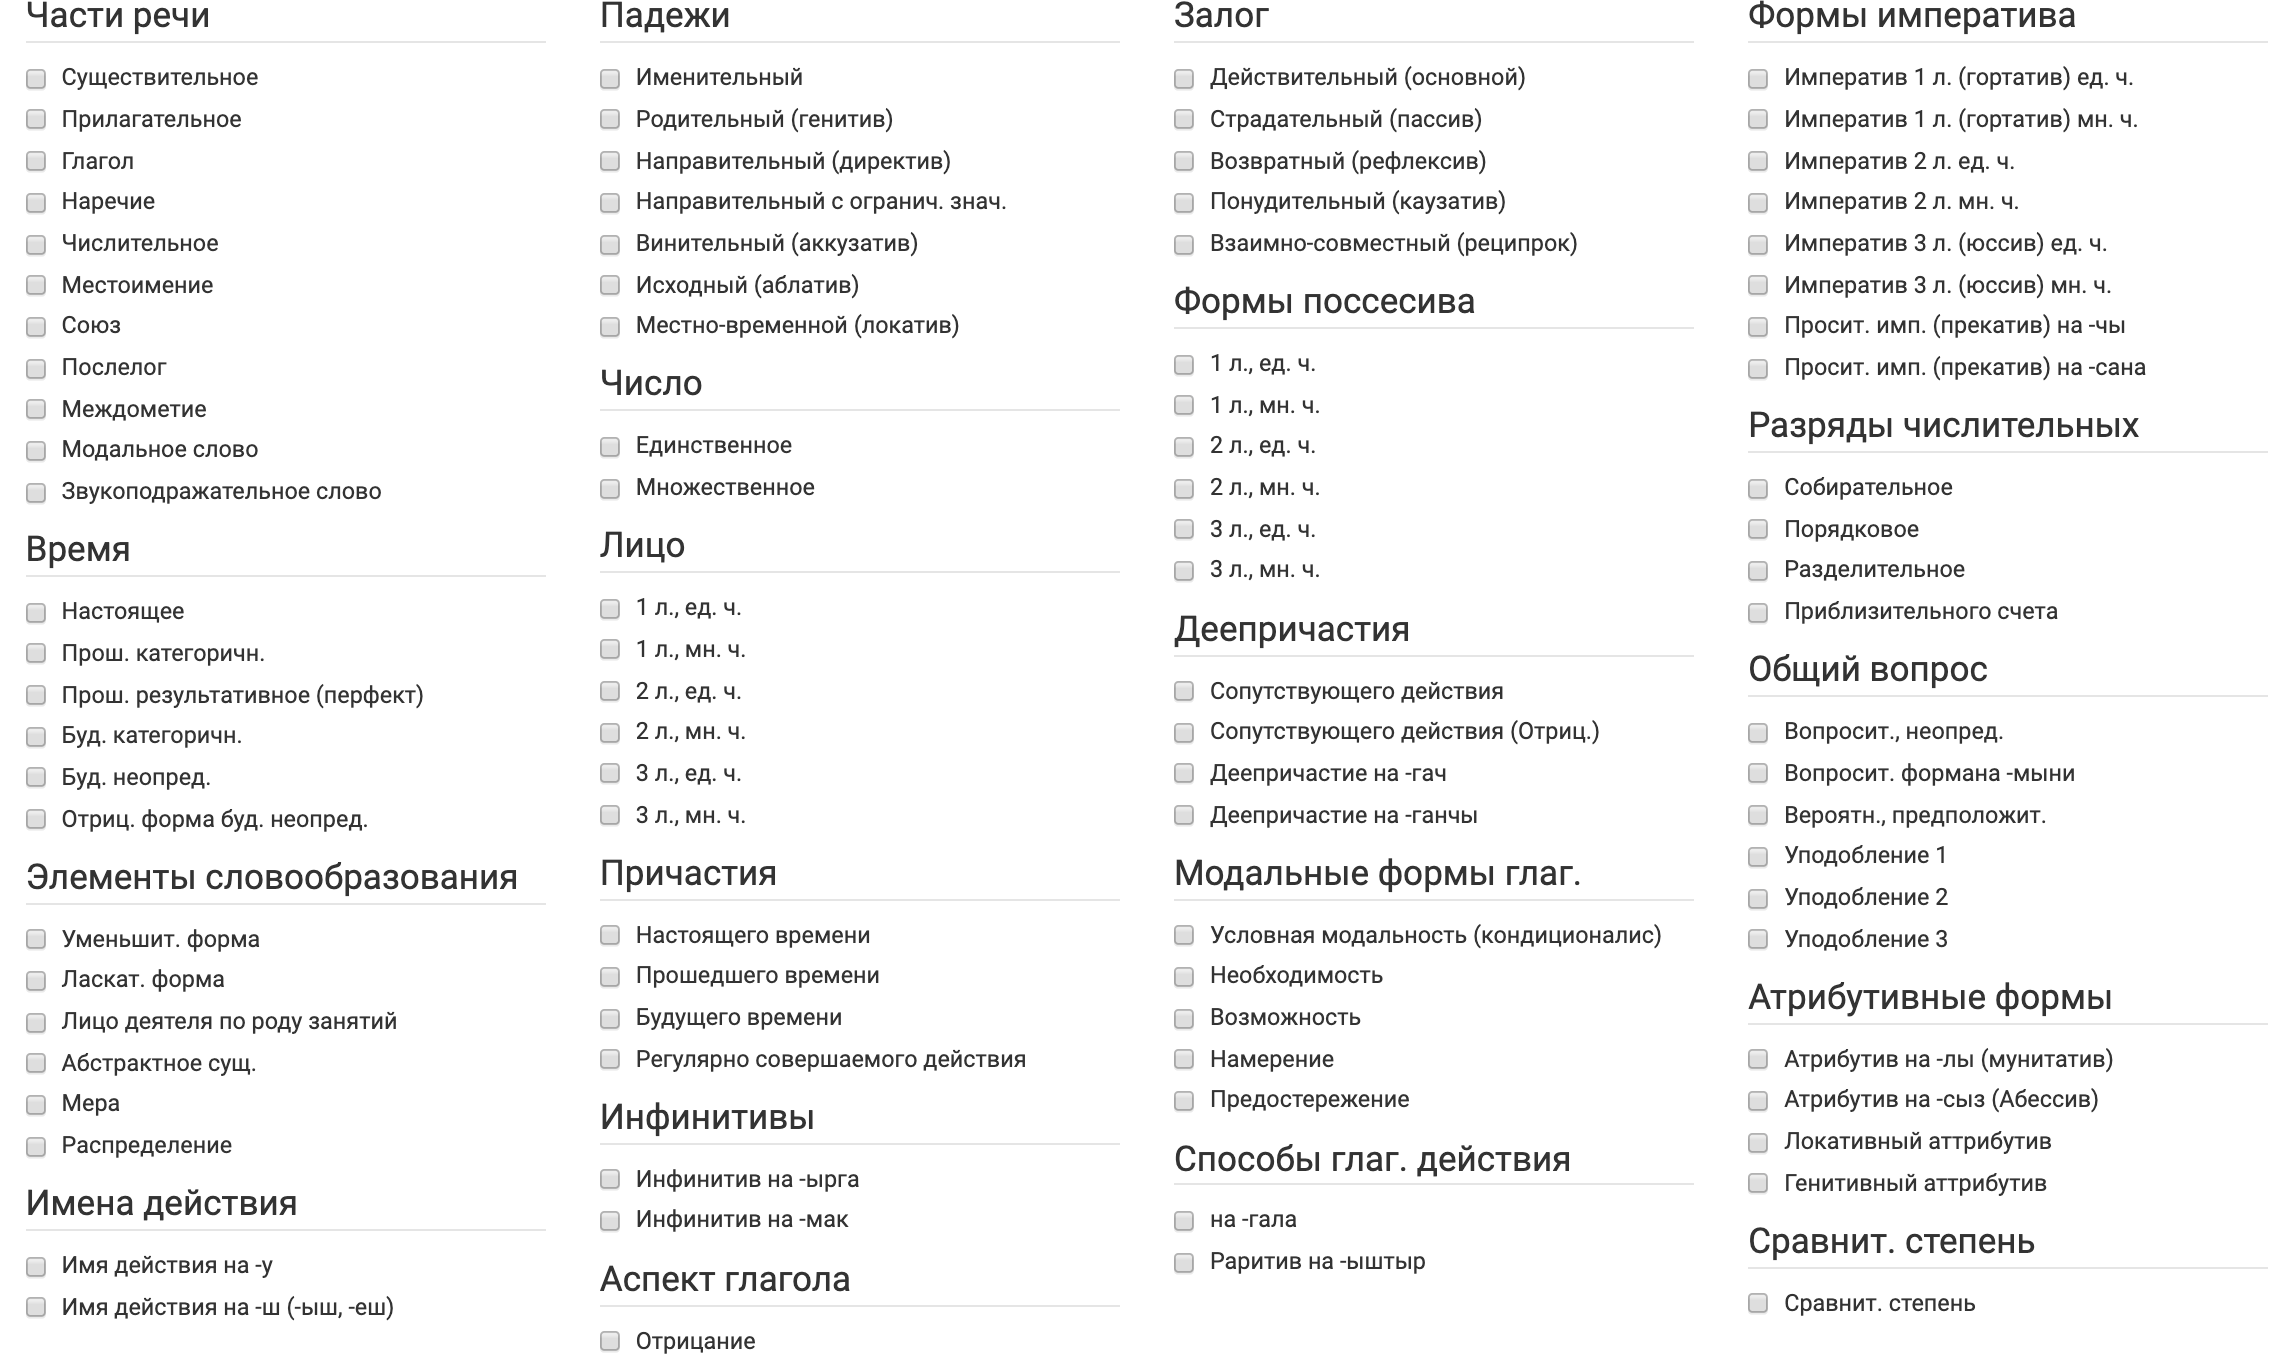
\includegraphics[width=\textwidth]{pics/tugan_tel_1}
\label{fig:tugan_tel_1}
\end{figure}

Судя по тому, что было в статье NER in Tatar, существует внутреннее IDE для выполнения автоматических запросов, которые сложно воспроизвести из-за отсутствия доступа (ну и доступа к любому коду статьи).

Теперь поговорим подробнее про корпус и про то, как он устроен.

Это .zip файл, состоящий из 7557 .txt файлов, в общей сложности весом 1 183 023 978 Б. Как уже упоминалось ранее, корпус Туган Тел автоматически размечен с помощью программного инструментарии PC-KIMMO и, как водится для автоматической разметки, она далеко неидеальная. 

*TODO: показать пример разметки*

Первое слово в каждом файле распознано как Error, все русские слова не распознаны (а их в татарском языке некоторое ненулевое количество, так как происходит какое-то достаточное количество заимствований). К сожалению для меня, очень часто русскоязычные слова оказывались как раз именованными сущностями, такими как, например, названия улиц, но распознаны они были как Error, что очень печально.

*TODO: написать \% Error от общего количества слов и привести пару примеров*

В этом файле огромная куча всяких тегов, про которые без бутылки не разберешься (и даже гугление этого парсера, блин, не помогает). Но эмпирическим методом было выяснено, что атрибут PROP --- это как раз та самая именованная сущность, что нам нужна. На основании этого все остальные атрибуты были выброшены, а PROP заменен на B-PER, так как используемая модель использовала IOB метод разметки (TODO: написать про IOB метод разметки).

Всего в текстах 30 753 824 слов, из них 534 514 это автоматически размеченные именованные сущности, что составляет $1,738\%$ от всех слов. 

*TODO: привести примеры слов с атрибутом PROP*.

*TODO: подсчитать, раз в сколько предложений в среднем встречается именованная сущность*

Также в качестве корпуса текста есть татарская википедия. На данный момент она содержит 89 252 статей, причём некоторые из них сгенерированы автоматически, что ухудшает качество текстов как корпуса для обучения, так как некоторые фразы становятся частотными не из-за того, что они действительно часто используются в языке, а из-за множества сгенерированных статей. *TODO вставить пример про бассейны*

Проблема с татарской википедией также была в смеси латиницы и кириллицы *TODO экскурс в историю по поводу того, как мы до такой жизни дошли*, так что пришлось ещё и из латиницы в кириллицу переводить.


\subsection{Обучение и тюнинг моделей}

\subsubsection{BiLSTM-CRF}

Была использована модель BiLSTM-CRF, которая норм заработала. Она использует разметку IOB, так что данные пришлось немного подкорректировать и добавить данную разметку. Весь морфологический разбор, кроме разметки именованных сущностей, никак не используется. Из-за того, что у меня нет мощностей для вычислений, приходилось обучаться не на всей выборке, а только на части. Модель показала очень хороший результат.

\medskip

\begin{tabular}{| l | l | l | l | l | l | l |}
\hline
Category               & Precision  &   Recall   &  F-score   &  Predicts  &   Golds    &  Correct   \\

\hline
 PER                                 & 99.768     & 90.727     & 95.033     & 2589       & 2847       & 2583       \\
\hline
\end{tabular}



*TODO: описание модели*

\subsubsection{BERT}

BERT есть для татарского языка, так что осталось его только запустить, что я ещё не сделала, но планирую вот уже на этой неделе. TODO: описать BERT.


\section{Воспроизведение статьи Невзоровой}

Была воспроизведена статья Невзоровой, на министерствах действительно показала хорошие результаты, но стало очевидно, что это полуручная история, потому что мусор пришлось выкидывать в ручном режиме. Ну и не удалось воспроизвести запросы в Туган Тел, а поиск был возможен только по слову (фразе). С помощью этого результата хочется разметить википедию, на википедии обучиться, а потом попытаться протестировать на Туган Тел и сравнить результаты.

\section{Сравнение результатов}

В процессе.


